\documentclass{../../text-style}

\texttitle{Лекция 1: О программной инженерии}

\begin{document}

\maketitle
\thispagestyle{empty}

\attribution{Тимофей Александрович Брыксин, бывш. доцент кафедры системного программирования СПбГУ}

\section{Введение}

Большая часть программ, за которые люди готовы платить деньги, довольно сложна. Даже небольшое по промышленным меркам приложение требует порядка двух-трёх человеко-лет на разработку и имеет размер в несколько десятков тысяч строк кода. Большие программные системы\footnote{См. \url{http://www.informationisbeautiful.net/visualizations/million-lines-of-code/}.} могут иметь несколько миллионов строк кода и занимать сотни и тысячи человеко-лет разработки. При этом каждый из вас понимает, что может писать гораздо больше 100 строчек кода в день\footnote{См. \url{http://stackoverflow.com/questions/966800/mythical-man-month-10-lines-per-developer-day-how-close-on-large-projects}}, а <<за выходные>> вообще может сделать практически всё. Тут весь вопрос в том, что же по факту создаётся.

\begin{center}
    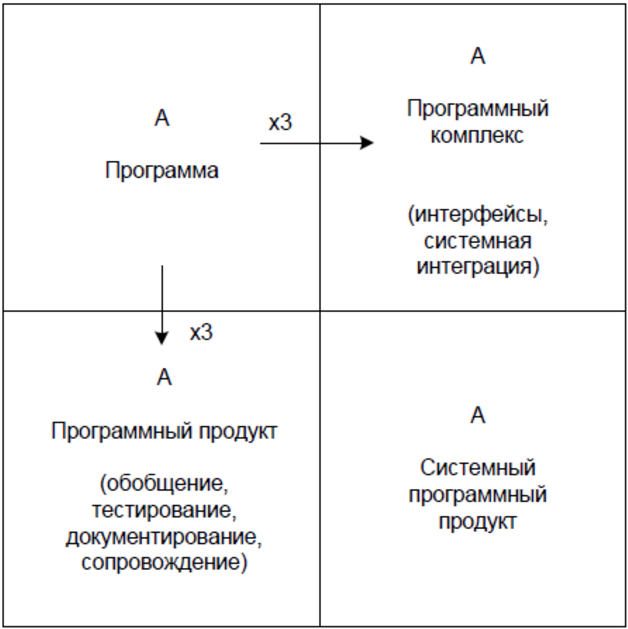
\includegraphics[width=0.5\textwidth]{brooksSquare.png}
\end{center}

На картинке выше (книга Брукса\footnote{Ф. Брукс, Мифический человеко-месяц, или Как создаются программные системы. 2021г, 368 С.} хоть и устарела местами, но во многом не теряет своей актуальности) слева вверху показана программа~--- законченный кусок кода, который его автор может скомпилировать, запустить на своем устройстве и который выполняет нужную задачу. Это именно то, чем неопытные программисты привыкли оценивать свою производительность. Но за такой код мало кто готов платить или использовать его в своих проектах.

При перемещении по стрелке вниз программа превращается в программный продукт. Это программа, которую любой человек может запускать, тестировать, исправлять и развивать. Она может использоваться в различных операционных средах и со многими наборами данных. Чтобы стать общеупотребительным программным продуктом, программа должна быть написана в обобщенном стиле. В частности, диапазон и вид входных данных должны быть настолько обобщенными, насколько это допустимо. Затем программу нужно тщательно протестировать, чтобы быть уверенным в ее надежности. Для этого нужно подготовить достаточное количество контрольных примеров для проверки диапазона допустимых значений входных данных и определения его границ, обработать эти примеры и зафиксировать результаты. Приложению нужен хороший пользовательский интерфейс, который нужно будет ещё разработать. Наконец, развитие программы в программный продукт требует создания подробной документации, с помощью которой каждый мог бы использовать ее, делать исправления и расширять. Ну и сама программа должна быть написана так, чтобы её потенциально можно было адекватно расширять и сопровождать\footnote{См. \url{https://en.wikipedia.org/wiki/Write-only_language}.}. По разным эмпирическим оценкам программный продукт стоит в 3-10 раз дороже, чем просто отлаженная программа с такой же функциональностью. 

При пересечении вертикальной границы программа становится компонентом программного комплекса. Последний представляет собой программную систему, в состав которой входит набор взаимодействующих программ, согласованных по программным интерфейсам и форматам данных, и все вместе решающие какие-то более сложные задачи, чем каждая по отдельности. Хорошим примером тут можно считать консольные утилиты *nix. Чтобы стать частью программного комплекса, синтаксис и семантика ввода и вывода программы должны удовлетворять точно определенным интерфейсам. Программа должна быть также спроектирована таким образом, чтобы использовать заранее оговоренный объём ресурсов~--- объем памяти, устройства ввода/вывода, процессорное время. Наконец, программу нужно протестировать вместе с прочими системными компонентами во всех сочетаниях, которые могут встретиться. Это тестирование может оказаться большим по объему, поскольку количество тестируемых случаев растет экспоненциально. Оно также занимает много времени, так как скрытые ошибки выявляются при неожиданных взаимодействиях отлаживаемых компонентов. Компонент программного комплекса стоит примерно так же в 3-10 раз дороже, чем автономная программа с теми же функциями. И этот порядок может увеличиться, если в системе много компонентов. 

Так чем программирование отличается от разработки коммерческих проектов? Для начала, первое является некоторой абстрактной деятельностью и может происходить во многих различных контекстах. Можно программировать для того, чтобы собственно научиться программировать (например, на занятиях в университете), для удовольствия (например, сделать игру и играть в неё с друзьями), можно программировать в рамках научных разработок (например, в рамках исследований в биоинформатике или лингвистике). А вот промышленное программирование, как правило, происходит в команде (уж больно большие получаются проекты, чтобы делать их в одиночку), и совершенно точно~--- для заказчика, который платит за работу деньги. При этом необходимо точно понимать, что нужно заказчику, выполнить работу в определенные сроки и результат должен быть нужного качества~--- того, которое удовлетворит заказчика и за которое он заплатит. Чтобы удовлетворить этим дополнительным требованиям, программирование <<обрастает>> различными дополнительными видами деятельности.

Разработка программного кода предваряется анализом и проектированием. Трудозатраты на анализ и проектирование, а также форма представления их результатов сильно варьируются от видов проектов и предпочтений разработчиков и заказчиков. А до этого нужно ещё собрать и проанализировать требования и пожелания к продукту. Требуются также специальные усилия по организации процесса разработки. Например, сейчас популярна итеративно-инкрементальная модель, когда требуемая функциональность создается порциями, которые менеджеры и заказчик могут оценить, и тем самым есть возможность управления ходом разработки. Однако эта общая модель имеет множество модификаций и вариантов. А ведь есть ещё и другие модели.

Разработку системы также необходимо выполнять с учетом удобств ее дальнейшего сопровождения, повторного использования и интеграции с другими системами. Это значит, что система разбивается на компоненты, удобные в разработке, годные для повторного использования и интеграции. А также имеющие необходимые характеристики по быстродействию. Для этих компонент тщательно прорабатываются интерфейсы. Сама же система документируется на многих уровнях, создаются правила оформления программного кода, то есть проводится дополнительная работа, помогающая создать и поддерживать единую, стройную архитектуру, единообразный стиль, порядок в коде.

Нужно выбрать, какие технологии мы будем использовать. Нужно спланировать, как будет организован процесс разработки: какие нам нужны люди, в какой момент подключать их к работе, какого уровня специалисты нам нужны, нужно ли покупать какой-то софт, нужна ли аренда офиса, какие в проекте будут команды, как они будут организованы, как будет строиться их взаимодействие, как оценивать успешность хода работ, что делать, если возникли непредвиденные сложности, как работать с поступающими изменениями, как контролировать качество продукта, как наладить его выпуск и развёртывание, как будет организовано сопровождение и многое-многое другое.

Все эти и другие дополнительные виды деятельности, выполняемые в процессе промышленного программирования и необходимые для успешного выполнения заказов и будем называть программной инженерией (software engineering). Получается, что так мы обозначаем, во-первых, некоторую практическую деятельность, а во-вторых, специальную область знания. Или другими словами, научную дисциплину. Ведь для облегчения выполнения каждого отдельного проекта, для возможности использовать разнообразный положительный опыт, достигнутый другими командами и разработчиками, этот самый опыт подвергается осмыслению, обобщению и надлежащему оформлению. Так появляются различные методы и практики (best practices)~--- тестирования, проектирования, работы над требованиями, архитектурных шаблонов и пр. А также стандарты и методологии, касающиеся всего процесса в целом. Вот эти-то обобщения и входят в программную инженерию как в область знания.

Итого, в сферу программной инженерии попадают все вопросы и темы, связанные с организацией и улучшением процесса разработки ПО, управлением коллективом разработчиков, разработкой и внедрением программных средств поддержки жизненного цикла разработки ПО. 

Необходимость в программной инженерии как в специальной области знаний была осознана мировым сообществом в конце 60-х годов прошлого века. Рождением программной инженерии является 1968 год~--- конференция NATO Software Engineering, г. Гармиш (ФРГ), которая целиком была посвящена рассмотрению этих вопросов, и которая была спровоцирована поиском решений для происходившего в то время <<кризиса программного обеспечения>>.

Причины кризиса программного обеспечения были связаны с общей сложностью аппаратного обеспечения и сложностью разработки программного обеспечения. Как сказал по этому поводу Э. Дейкстра, <<[The major cause of the software crisis is] that the machines have become several orders of magnitude more powerful! To put it quite bluntly: as long as there were no machines, programming was no problem at all; when we had a few weak computers, programming became a mild problem, and now we have gigantic computers, programming has become an equally gigantic problem>>.

Кризис проявляет себя самым различным образом:
\begin{itemize}
    \item стоимость проектов превышает бюджет,
    \item в проектах превышаются сроки выполнения,
    \item программное обеспечение было слишком неэффективным,
    \item программное обеспечение имело слишком низкое качество,
    \item программное обеспечение зачастую не отвечало необходимым требованиям,
    \item проекты были неуправляемыми, и возникали трудности с поддержкой кода,
    \item программное обеспечение было непригодным для распространения.
\end{itemize}

Колоссальные успехи в области развития средств вычислительной техники пришли в противоречие с низкой производительностью труда программистов и низкими темпами ее роста. В связи с усложнением бизнеса, усложнением программных систем стало очевидным, что их трудно проектировать, кодировать, тестировать и особенно трудно понимать, когда возникает необходимость их модификации в процессе сопровождения. Появилась жизненная потребность в создании технологии разработки программных средств и инженерных методов их проектирования для существенного улучшения производительности труда разработчиков.

Впрочем, как показывает таблица ниже, люди до сих пор не имеют проверенного и надёжного способа создавать качественное ПО в срок и в рамках зафиксированного бюджета. И чем сложнее проект, тем сложнее довести его до конца.

\begin{center}
    \begin{tabu} {| X[2 l p] | X[1 c p] | X[1 c p] | X[1 c p] | X[1 c p] | X[1 c p] |}
        \tabucline-
        \everyrow{\tabucline-}
                            & 2011 & 2012 & 2013 & 2014 & 2015 \\
        Successful          & 29\% & 27\% & 31\% & 28\% & 29\% \\
        Challenged          & 49\% & 56\% & 50\% & 55\% & 52\% \\
        Failed              & 22\% & 17\% & 19\% & 17\% & 19\% \\
    \end{tabu}
\end{center}

Почему же до сих пор так всё плохо в индустрии разработки ПО? Одна из самых главных причин~--- сложность ПО. Сложность программных объектов зависит от их размеров в гораздо большей степени, чем для любых других создаваемых человеком объектов. Разрабатывать сложное ПО невыразимо трудно. В сложных системах огромное количество компонент, которые могут сочетаться друг с другом неким нелинейным способом, генерируя ещё большее количество сочетаний, и сложность целого растет значительно быстрее, чем линейно. К тому же масштабирование программного объекта~--- это не просто увеличение в размере или количестве каких-то типовых элементов, это обязательно увеличение числа различных элементов. В итоге программные системы очень сложно разрабатывать, понимать, описывать, тестировать. 

Сложность программ является существенным, а не второстепенным свойством. Поэтому описания программных объектов, абстрагирующиеся от их сложности, часто абстрагируются от их сущности. Математика и физические науки за три столетия достигли больших успехов, создавая упрощенные модели сложных физических явлений, получая из этих моделей свойства и проверяя их опытным путем. Это удавалось благодаря тому, что сложности, игнорировавшиеся в моделях, не были существенными свойствами явлений. И это не действует, когда сложности являются сущностью. Многие классические трудности разработки программного обеспечения проистекают из этой сложности сущности и ее нелинейного роста при увеличении размера. Сложность служит причиной трудности процесса общения между участниками команды разработчиков, что ведет к ошибкам в продукте, превышению стоимости разработки, затягиванию выполнения графиков работ. Сложность служит причиной трудности перечисления, а тем более понимания, всех возможных состояний программы, а отсюда возникает ее ненадежность. Сложность функций служит причиной трудностей при их вызове, из-за чего программами трудно пользоваться. Сложность структуры служит причиной трудностей при развитии программ и добавлении новых функций так, чтобы не возникали побочные эффекты. Сложность структуры служит источником невизуализуемых состояний, в которых нарушается система защиты. Сложность служит причиной не только технических, но и административных проблем. Из-за сложности трудно осуществлять контроль, в результате страдает концептуальная целостность. Трудно найти и держать в голове все <<движущиеся части>> системы. 

Вторая причина~--- недостаток накопленного у человечество опыта. Программная инженерия~--- весьма молодая область знаний, и практически на наших глазах происходит формирование многих её частей. Возможно, через несколько сотен лет создание ПО станет настолько же понятным и отработанным процессом, как строительство зданий, но сейчас эта деятельность всё ещё больше похожа на творчество, чем на ремесло, и довольно плохо прогнозируется. В результате предсказать результат часто бывает крайне непросто.

Третий момент состоит в том, что программные объекты постоянно подвержены изменениям, в том числе (в отличие от большинства объектов физического мира) и уже после их изготовления. Программы часто меняются, потому что 1) это становится необходимо (исправляются ошибки или меняется понимание их предназначения или окружающей инфраструктуры) и 2) это в принципе возможно за невысокую цену (тут как повезёт, на самом деле~--- часто заказчику бывает тяжело объяснить, что для реализации такой-то фичи придётся половину кода переписывать). Программы~--- это продукт мысли, воплощённый в программном коде. Поменяв несколько символов текста и осуществив процедуру сборки (и, возможно, размещения) программы, мы можем получить абсолютно другое поведение, чем у этой программы было раньше. И всё это чаще всего в полностью автоматическом режиме и практически без каких-либо затрат. Со многими физическими объектами такого в принципе осуществить невозможно, а если и возможно, это может быть очень долго и дорого. Да, здания тоже перестраиваются, но если бы можно было бы поменять внешний вид или добавить своему дому пару лишних этажей простым нажатием клавиш, вид наших улиц бы сильно преобразился. 

Ещё один момент, который стоит отметить в разработке ПО~--- сильная социальная составляющая проектов. Программные продукты разрабатываются людьми (разработчиками) для людей (заказчиков). Должно быть много социального взаимодействия, как внутри команды, так и с людьми снаружи. В состав команды входят разные люди, которые выполняют разные работы, и данный курс будет частично направлен на то, чтобы показать, чем же ещё нужно заниматься, чтобы уверенно вести программные проекты к завершению.

\begin{center}
    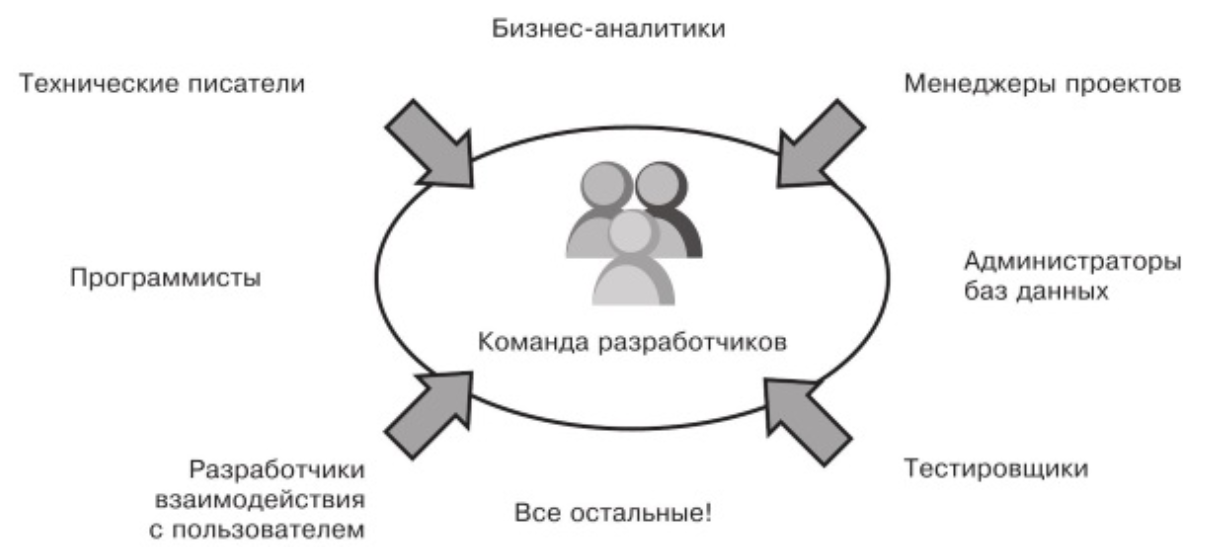
\includegraphics[width=0.5\textwidth]{team.png}
\end{center}

Успех программного проекта зачастую определяется социальными факторами, а роль технологии второстепенна. Есть немало примеров технически отсталых систем, которые работают и полезны заказчикам. Обратное, как правило, неверно. От системы, не приносящей пользы (ожидаемой или реальной), заказчик рано или поздно откажется независимо от того, насколько блестящей она является в техническом отношении.

В связи со всем этим на рынке труда востребованы программисты, умеющие работать в команде. Проводя интервью, кандидатов оценивают не только на наличие тех или иных знаний и навыков (разумеется, программист должен уметь писать хороший код), но оценивается также, насколько хорошо данный человек вольётся в существующих коллектив, сможет ли он строить эффективное взаимодействие с остальными участниками проекта. Для многих компаний это даже важнее: при должном уровне человека можно довольно быстро научить пользоваться практически любыми языками и технологиями, а вот психологическую несовместимость исправить практически невозможно.

Имеющиеся промышленные стандарты для профессии <<Программист>> (более старый\footnote{Стандарт АПКИТ 2007 года, \url{http://www.apkit.ru/files/programer.doc} (дата обращения: 09.02.2023).} и более новый\footnote{Профстандарт Министерства труда и социальной защиты 06.001, <<Программист>>, 2022 года \url{https://profstandart.rosmintrud.ru/obshchiy-informatsionnyy-blok/natsionalnyy-reestr-professionalnykh-standartov/reestr-professionalnykh-standartov/index.php?ELEMENT_ID=115615} (дата обращения: 09.02.2023).}) подтверждают эти мысли:

\emph{Возрастает значение профессиональных компетенций коллективной разработки программного обеспечения, знание современных направлений, методов и технологий разработки программного обеспечения: 
    \begin{itemize}
        \item понимание обязанностей различных участников команды по разработке программного обеспечения: руководитель разработки программного обеспечения, руководитель технической группы (team leader), архитектор, программист, тестировщик, дизайнер, верстальщик, аналитик;
        \item владение современными стратегиями и технологиями организации коллективной разработки программного обеспечения, включая системы управления версиями, процессы непрерывной интеграции, стандарты оформления кода и методы инспекции кода;
        \item понимание основных направлений развития методов коллективной разработки, их отличий и целесообразности применения в зависимости от типа решаемых задач и требований организации;
        \item владение гибкими (Agile) методологиями разработки программных продуктов.
    \end{itemize}
}

Официальный профстандарт Минтруда 2022 года описывает четыре квалификационных уровня профессиональных программистов. Вообще, профстандарты, особенно новые, вышедшие после 2020 года, довольно грамотно составлены, и туда реально стоит посматривать, чтобы понимать, что от вас будут ожидать на работе. Светлая цель профстандартов~--- определить набор трудовых функций и соответствующих им знаний, умений и навыков, которые будут ожидаться от человека, занимающего ту или иную должность. Чтобы можно было стандартизовать профессиональную сертификацию~--- грубо говоря, по выпуску из вуза вы получаете диплом, в котором говорится, что вы умеете то, то и то, это соответствует такому-то уровню квалификации такого-то профстандарта, поэтому смело идёте работать (в совсем уж идеальном мире~--- без собеседования, поскольку уровень ваших навыков уже оценен и подтверждён организацией, которой все доверяют). А когда поработали немного~--- идёте в сертификационный центр, сдаёте на более высокий уровень и получаете повышение. В реальности оно так не работает, конечно (пока?), но профстандарты вполне адекватно отражают взгляд в среднем по индустрии на идеального сотрудника.

Профстандарты вводят 9 уровней квалификации, от первого~--- выполнять стандартные операции, не требующие специального обучения (неквалифицированный труд), до девятого~--- <<ответственность за результаты труда на общероссийском или международном уровне, управление крупными техносистемами, генерация фундаментальных знаний>>. Начиная с шестого уровня требуется диплом бакалавра, с седьмого~--- диплом магистра, девятый уровень требует окончания аспирантуры. 

Так вот, низший уровень квалификации программиста в профстандарте 06.001~--- третий (<<Выполняются стандартные задачи, но решения могут приниматься на основе наработанного опыта. Требуются специальные знания (срок обучения – до 1-го года)>>). Это даже не требует среднего профессионального образования, поэтому <<обычных>> программистов по-хорошему должны готовить ПТУ, а не вузы. Максимальный уровень квалификации для программиста~--- шестой, для суперкрутых программистов бакалаврский диплом всё-таки нужен.

Что по профстандарту должен уметь делать программист:

\begin{itemize}
    \item Разработка и отладка программного кода (3-й уровень квалификации, условно <<script kiddie>>, выпускник многочисленных онлайн-академий).
    \begin{itemize}
        \item Формализация и алгоритмизация поставленных задач для разработки программного кода.
        \item Написание программного кода с использованием языков программирования, определения и манипулирования данными в базах данных.
        \item Оформление программного кода в соответствии с установленными требованиями.
        \item Работа с системой управления версиями программного кода.
        \item Проверка и отладка программного кода.
    \end{itemize}
    \item Проверка работоспособности и рефакторинг кода программного обеспечения (4-й уровень квалификации).
    \begin{itemize}
        \item Разработка процедур проверки работоспособности и измерения характеристик компьютерного программного обеспечения.
        \item Разработка тестовых наборов данных для проверки работоспособности компьютерного программного обеспечения.
        \item Проверка работоспособности компьютерного программного обеспечения.
        \begin{itemize}
            \item \emph{Да-да, тестировщик должен иметь большую квалификацию, чем программист.}
        \end{itemize}
        \item Рефакторинг, оптимизация и инспекция программного кода.
        \item Исправление дефектов программного кода, зафиксированных в базе данных дефектов.
        \item Осуществление сборки однородных программных модулей в программный проект.
    \end{itemize}
    \item Интеграция программных модулей и компонентов и проверка работоспособности выпусков программного продукта (5-й уровень квалификации).
    \begin{itemize}
        \item Разработка процедур интеграции программных модулей.
        \item Осуществление интеграции программных модулей и компонентов и проверки работоспособности выпусков программного продукта.
    \end{itemize}
    \item Разработка требований и проектирование программного обеспечения (6-й уровень квалификации).
    \begin{itemize}
        \item Анализ возможностей реализации требований к компьютерному программному обеспечению.
        \item Разработка технических спецификаций на программные компоненты и их взаимодействие.
        \item Проектирование компьютерного программного обеспечения.
    \end{itemize}
\end{itemize}

Как видим, собственно написание кода~--- это \emph{далеко} не единственное, что требуется от программистов, более того, это \emph{требующая самой низкой квалификации} часть работы. А ведь для разработки программного обеспечения нужны не только программисты. В частности, программа <<Технологии программирования>> СПбГУ ведёт подготовку в соответствии со следующими профстандартами (помимо 06.001 <<Программист>>): 

\begin{itemize}
    \item 06.003 <<Архитектор программного обеспечения>>;
    \item 06.004 <<Специалист по тестированию в области информационных технологий>>;
    \item 06.011 <<Администратор баз данных>>;
    \item 06.015 <<Специалист по информационным системам>>;
    \item 06.019 <<Технический писатель (специалист по технической документации в области информационных технологий)>>;
    \item 06.022 <<Системный аналитик>>;
    \item 06.026 <<Системный администратор информационно-коммуникационных систем>>;
    \item 06.028 <<Системный программист>>;
    \item 40.011 <<Специалист по научно-исследовательским и опытно-конструкторским разработкам>>;
    \item 40.057 <<Специалист по автоматизированным системам управления производством>>.
\end{itemize}

В этом курсе мы все трудовые функции всех этих уважаемых профессий, конечно, не затронем. Основное внимание будет уделено управлению проектами и взаимодействию разных членов команды, но немного обсудим и то, чем занимаются основные роли. Этот курс надо понимать как введение в профессию тимлида, но с уточнением~--- мы не ставим своей целью сделать из вас тимлида. Цель этого курса~--- сделать так, чтобы вы понимали, что \emph{и почему} хочет от вас тимлид, и сделать так, чтобы когда вы дослужитесь до тимлида, вы знали, что в принципе от вас нужно и что гуглить.

Кстати, насчёт <<что гуглить>>: есть замечательная книга Guide to the Software Engineering Body of Knowledge (SWEBOK Guide), который по сути кратко описывает весь накопленный в программной инженерии свод знаний. Крайне рекомендуется к ознакомлению и использованию в качестве справочника по мере появления у вас управленческих обязанностей.

\end{document}
